% 
% Lecture Template for ME3023 -  Measurements in Mechanical Systems - Tennessee Technological University
%
% Spring 2020 - Summer 2020
% Tristan Hill, May 07, 2020 - June 12, 2020 - July 08, 2020
% Lecture Module - Electrical Instruments
% Topic 3 - Solderless Breadboards
%


\documentclass[fleqn]{beamer} % for presentation (has nav buttons at bottom)

%\usepackage{/home/thill/courses/measurements/lectures/measurements_lectures}
\usepackage{/home/tntech.edu/thill/courses/measurements/lectures/measurements_lectures}



\author{ME3023 - Measurements in Mechanical Systems} % original formatting from Mike Renfro, September 21, 2004

\newcommand{\MNUM}{5\hspace{2mm}} % Module number
\newcommand{\TNUM}{4\hspace{2mm}} % Topic number 
\newcommand{\moduletitle}{Electrical Instruments}
\newcommand{\topictitle}{Tektronix TBS100C Oscilloscope Troubleshooting} 

\newcommand{\sectiontitleI}{Device Overview}
\newcommand{\sectiontitleII}{Reccomended Procudures and Settings}
\newcommand{\sectiontitleIII}{Common Issues and Solutions}
\newcommand{\sectiontitleIV}{Example}


% custom box
\newsavebox{\mybox}

\title{Lecture Module - \moduletitle}

\date{Mechanical Engineering\vspc Tennessee Technological University}

\begin{document}
	
	\lstset{language=MATLAB,basicstyle=\ttfamily\small,showstringspaces=false}
	
	\frame{\titlepage \center\begin{framed}\Large \textbf{Topic \TNUM - \topictitle}\end{framed} \vspace{5mm}}
	
	
	% Section 0: Outline
	\frame{
		\large \textbf{Topic \TNUM - \topictitle} \vspace{3mm}\\
		
		\begin{itemize}
			
			\item \sectiontitleI    \vspc % Section I
			\item \sectiontitleII 	\vspc % Section II
			\item \sectiontitleIII 	\vspc %Section III
			\item \sectiontitleIV 	\vspc %Section IV
			
		\end{itemize}
		
	}



\section{\sectiontitleI}

% Section I - Frame I:
\frame{  \small
\frametitle{\sectiontitleI}


\underline{Tektronix TBS 1000C:} \vspace{5mm}\\
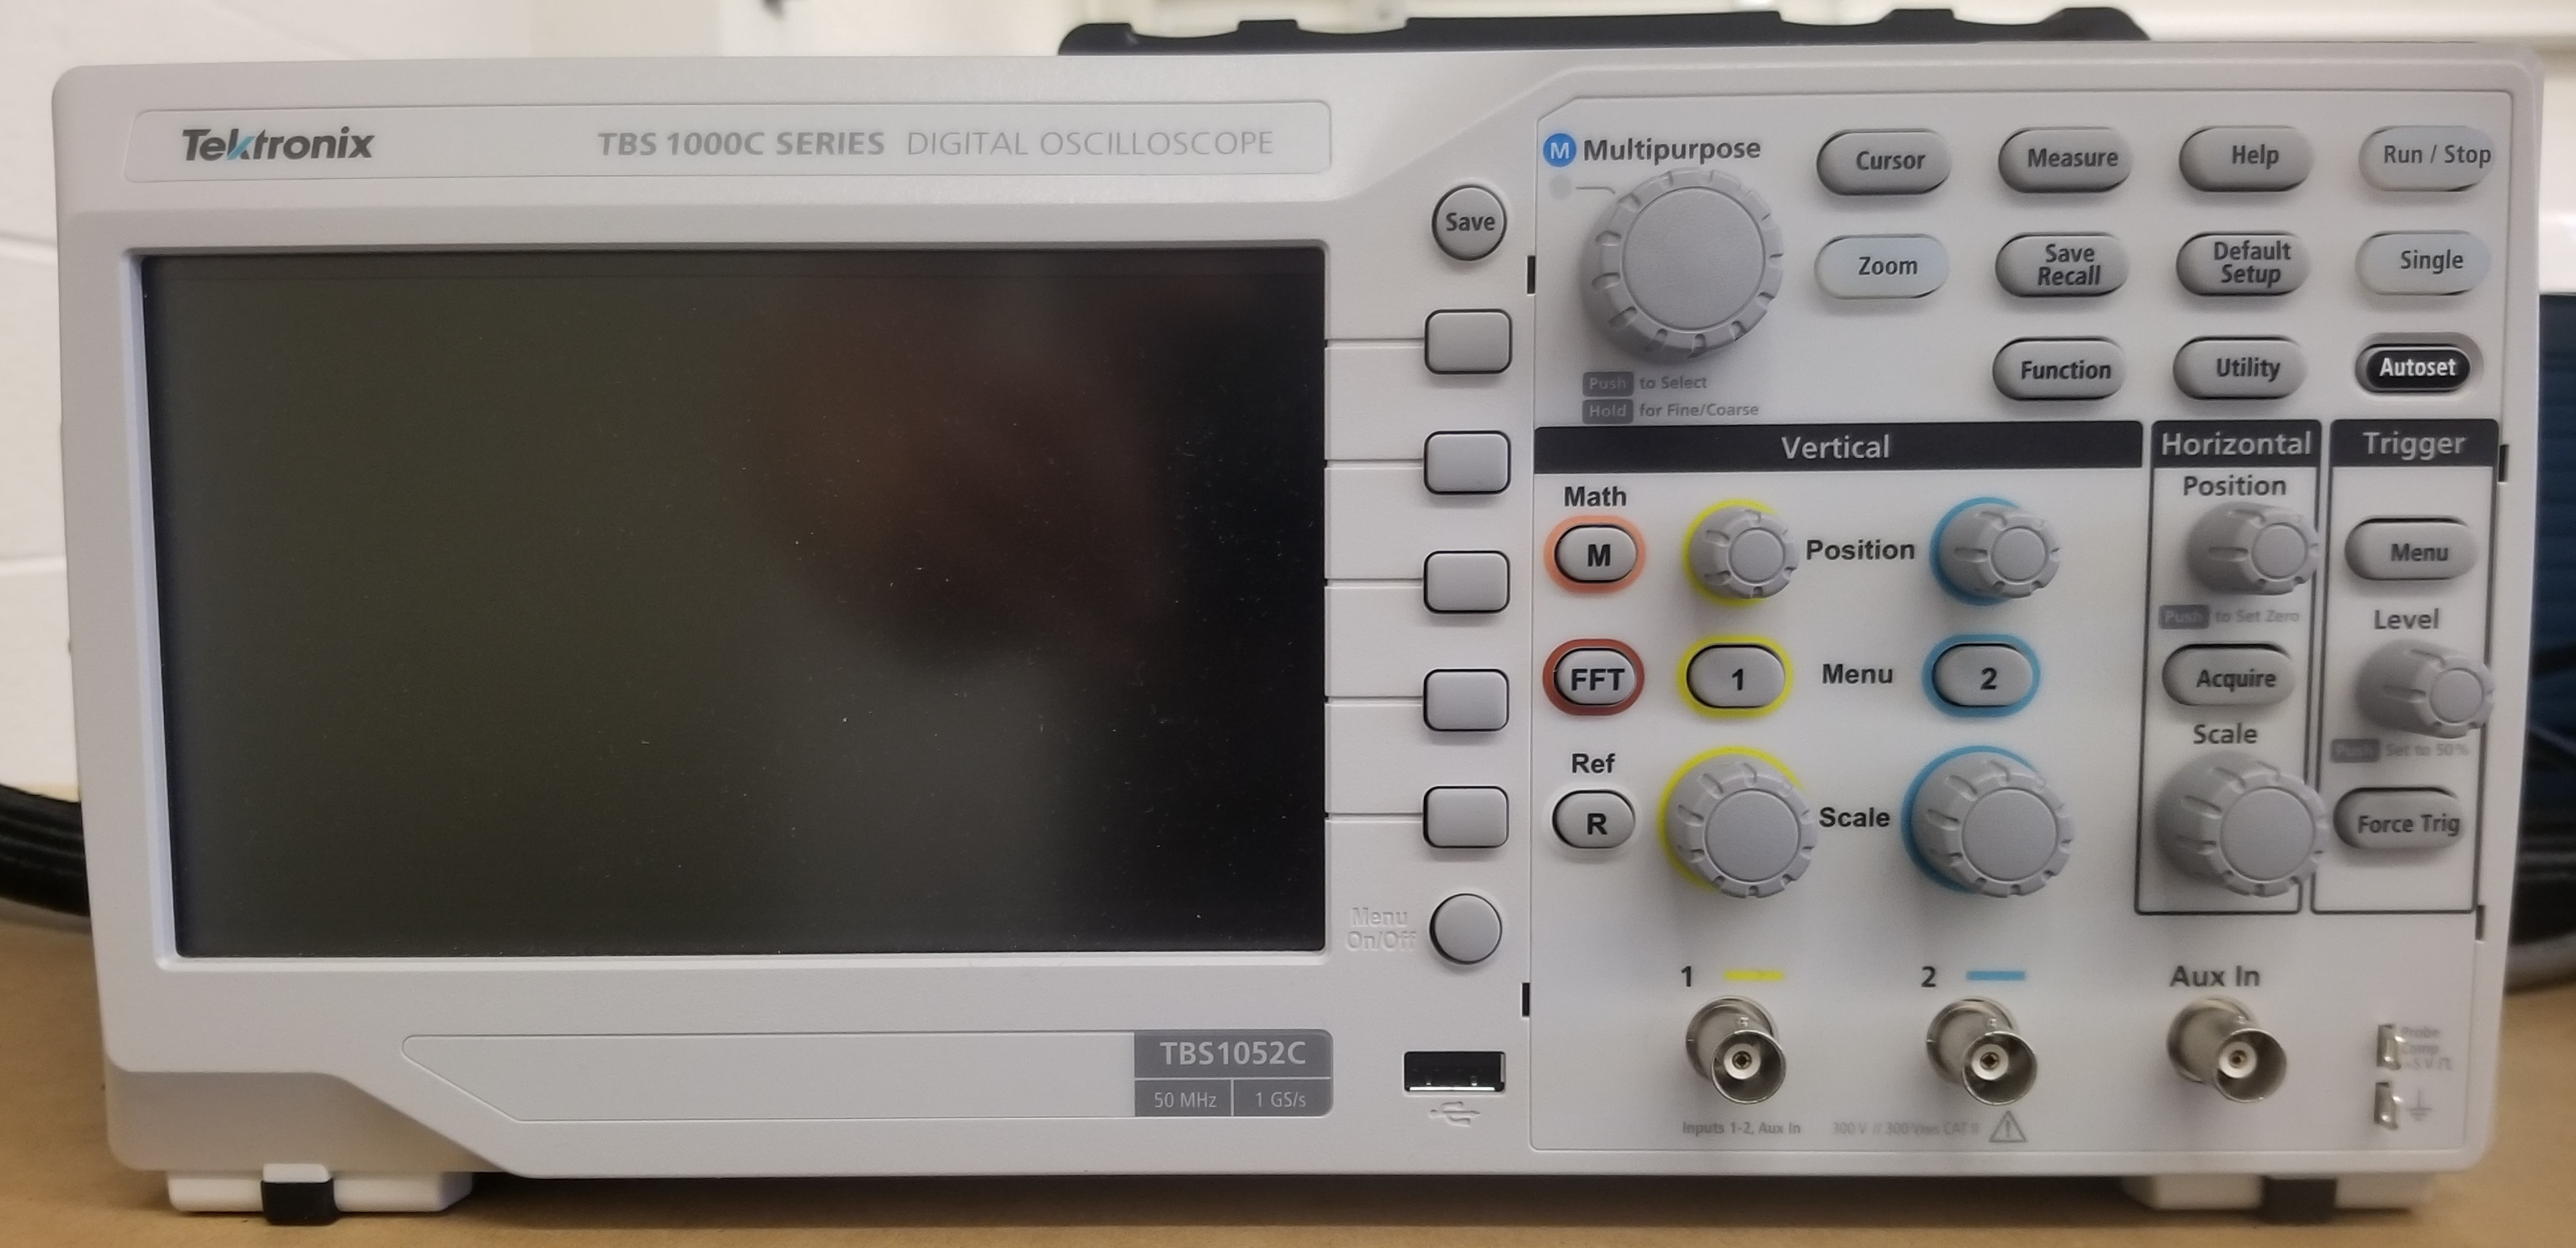
\includegraphics[scale=.065]{tektronix_tbs1000c_cropped.jpg}  \vspace{10mm}\\ 


}

% Section I - Frame II:
\frame{  \small
\frametitle{\sectiontitleI}

	

}


\section{\sectiontitleII}

% Section II - Frame I:
\frame{  \small
\frametitle{\sectiontitleII}
   
	

}

% Section II - Frame II:
\frame{  \small
\frametitle{\sectiontitleII}

		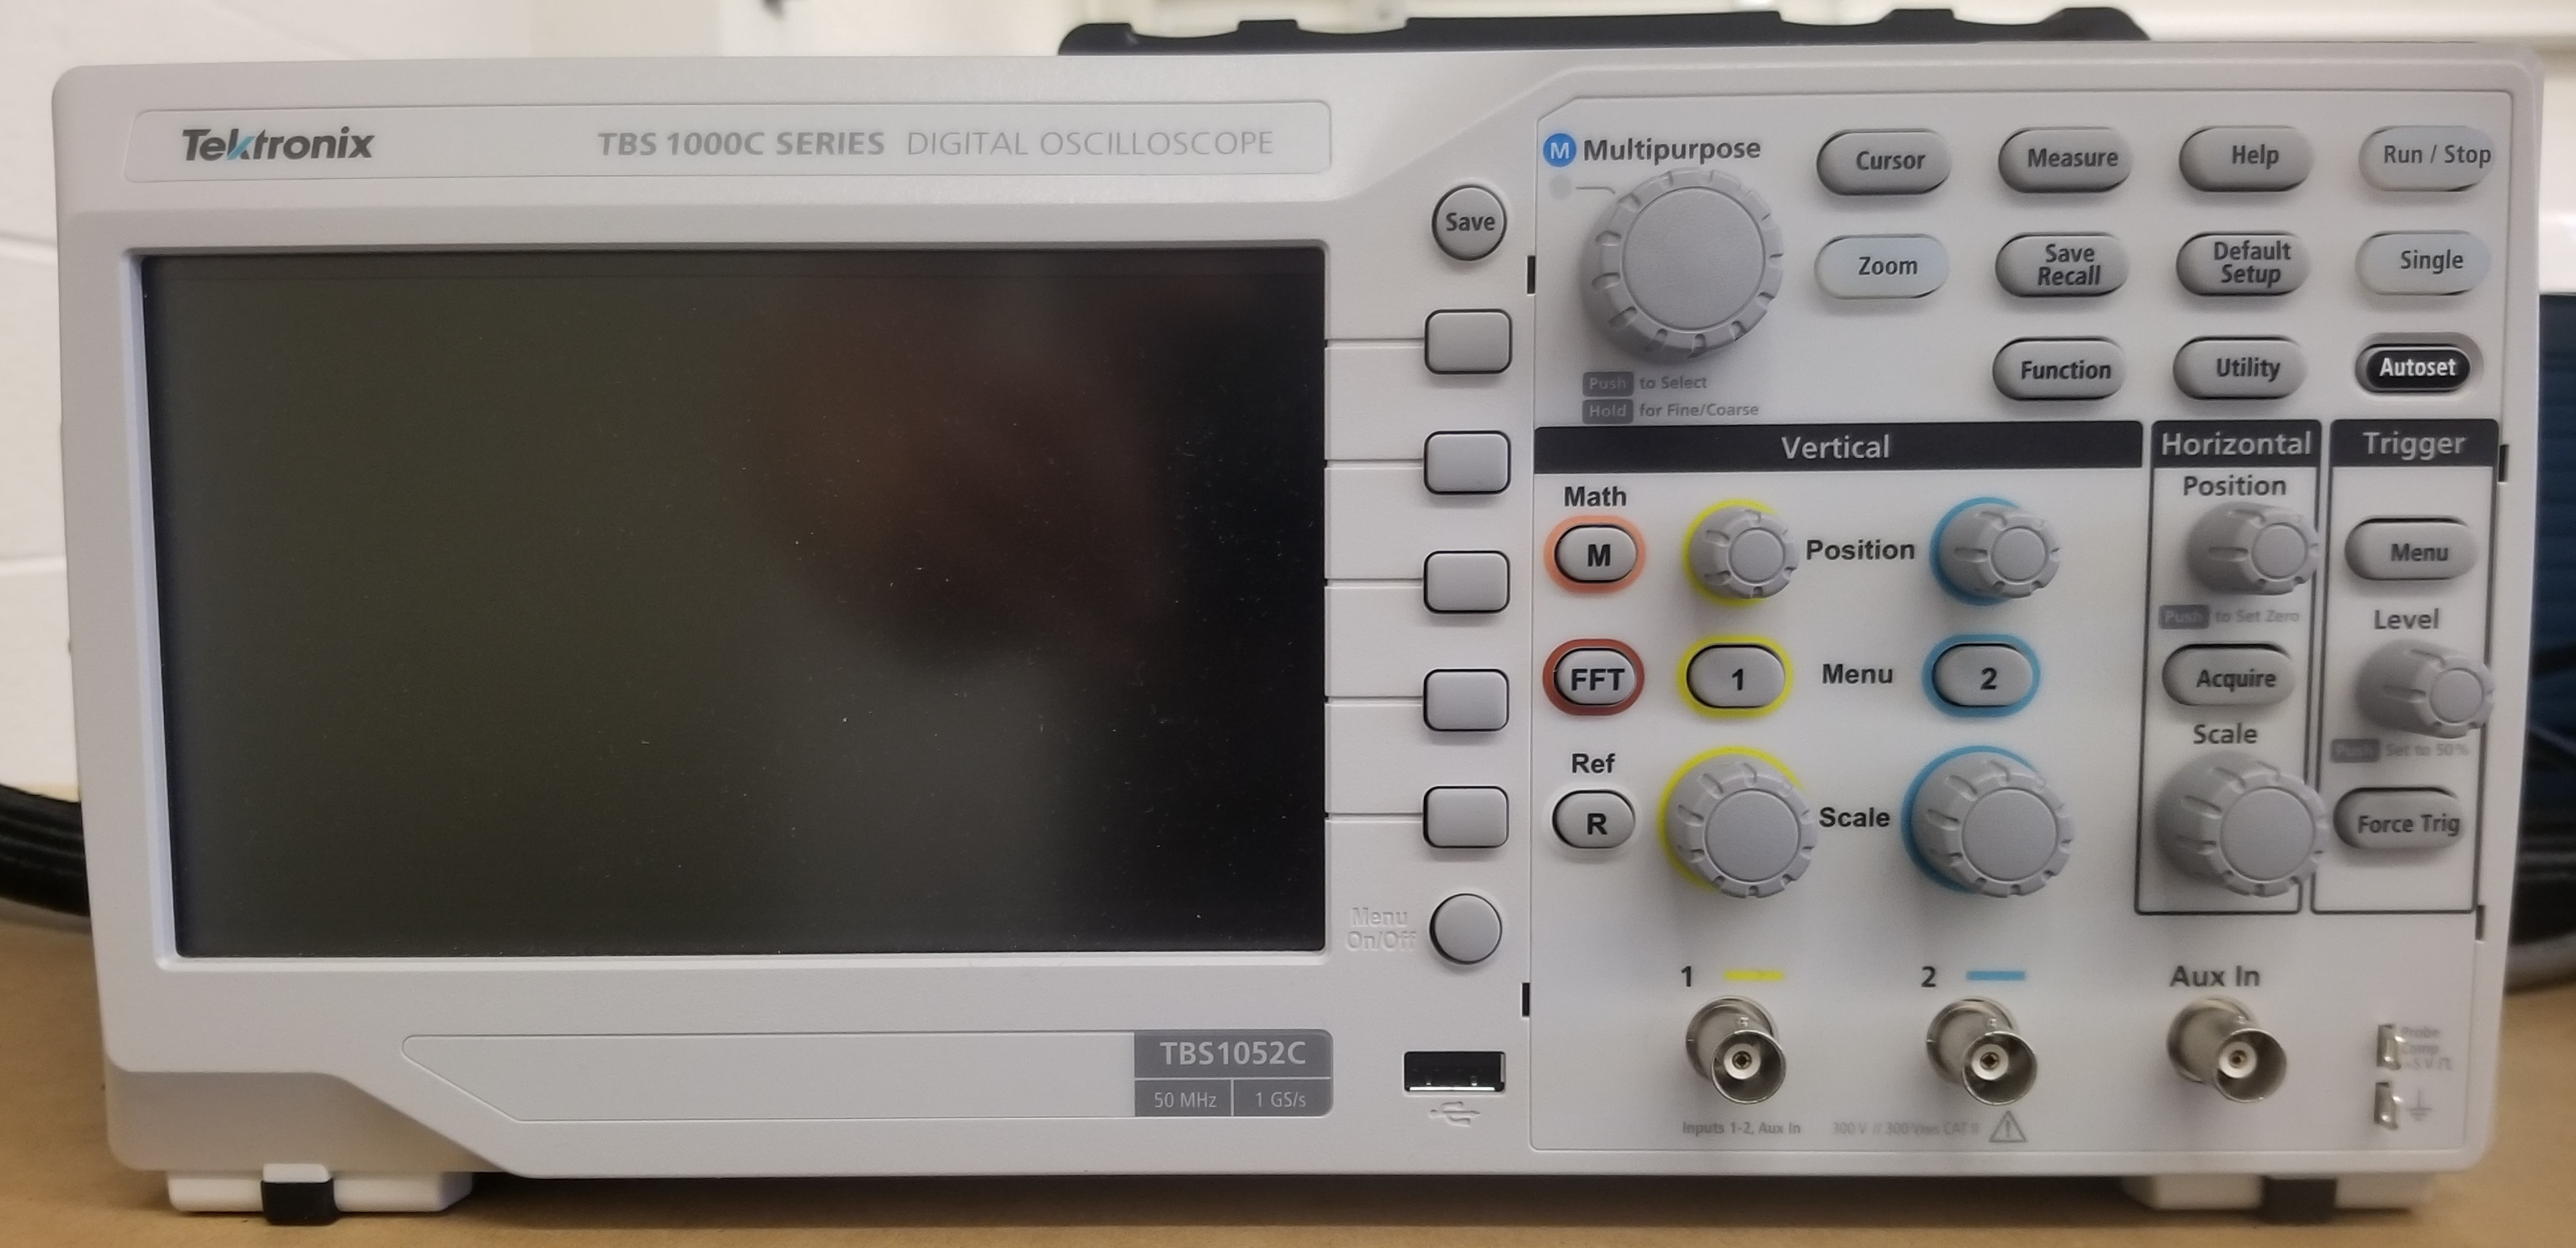
\includegraphics[scale=.075]{tektronix_tbs1000c_cropped.jpg} \vspace{10mm}\\

}

% Section II - Frame II:
\frame{  \small
\frametitle{\sectiontitleII}

		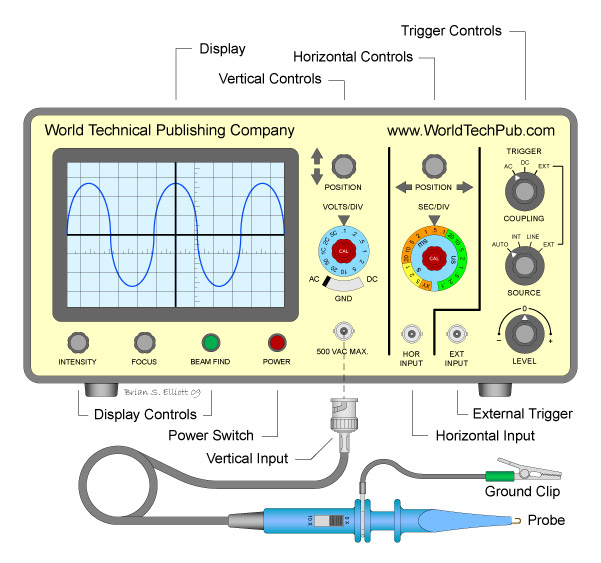
\includegraphics[scale=.5]{oscilloscope_fig1.jpg} \vspace{10mm}\\

}



\section{\sectiontitleIII}
	

	% Section III - Frame I:
	\frame{  \small
	\frametitle{\sectiontitleIII}

  }

  	% Section III - Frame II:
	\frame{  \small
	\frametitle{\sectiontitleIII}

  }


\section{\sectiontitleIV}

% Section IV - Frame I:
\frame{  \small
\frametitle{\sectiontitleIV}

%\begin{multicols}{2}

Example: 

%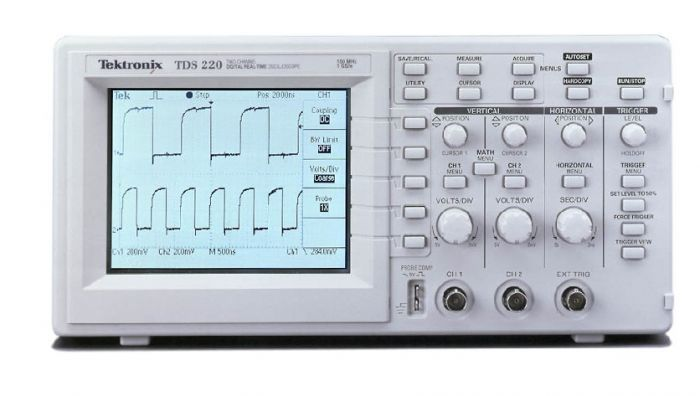
\includegraphics[scale=.35]{tds220.jpg}
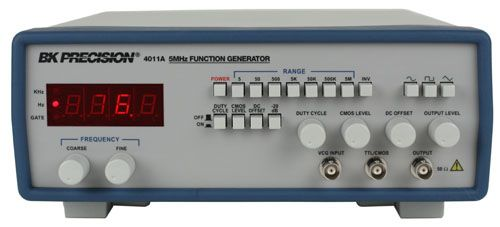
\includegraphics[scale=.35]{fn_gen.jpg} \hspace{15mm} 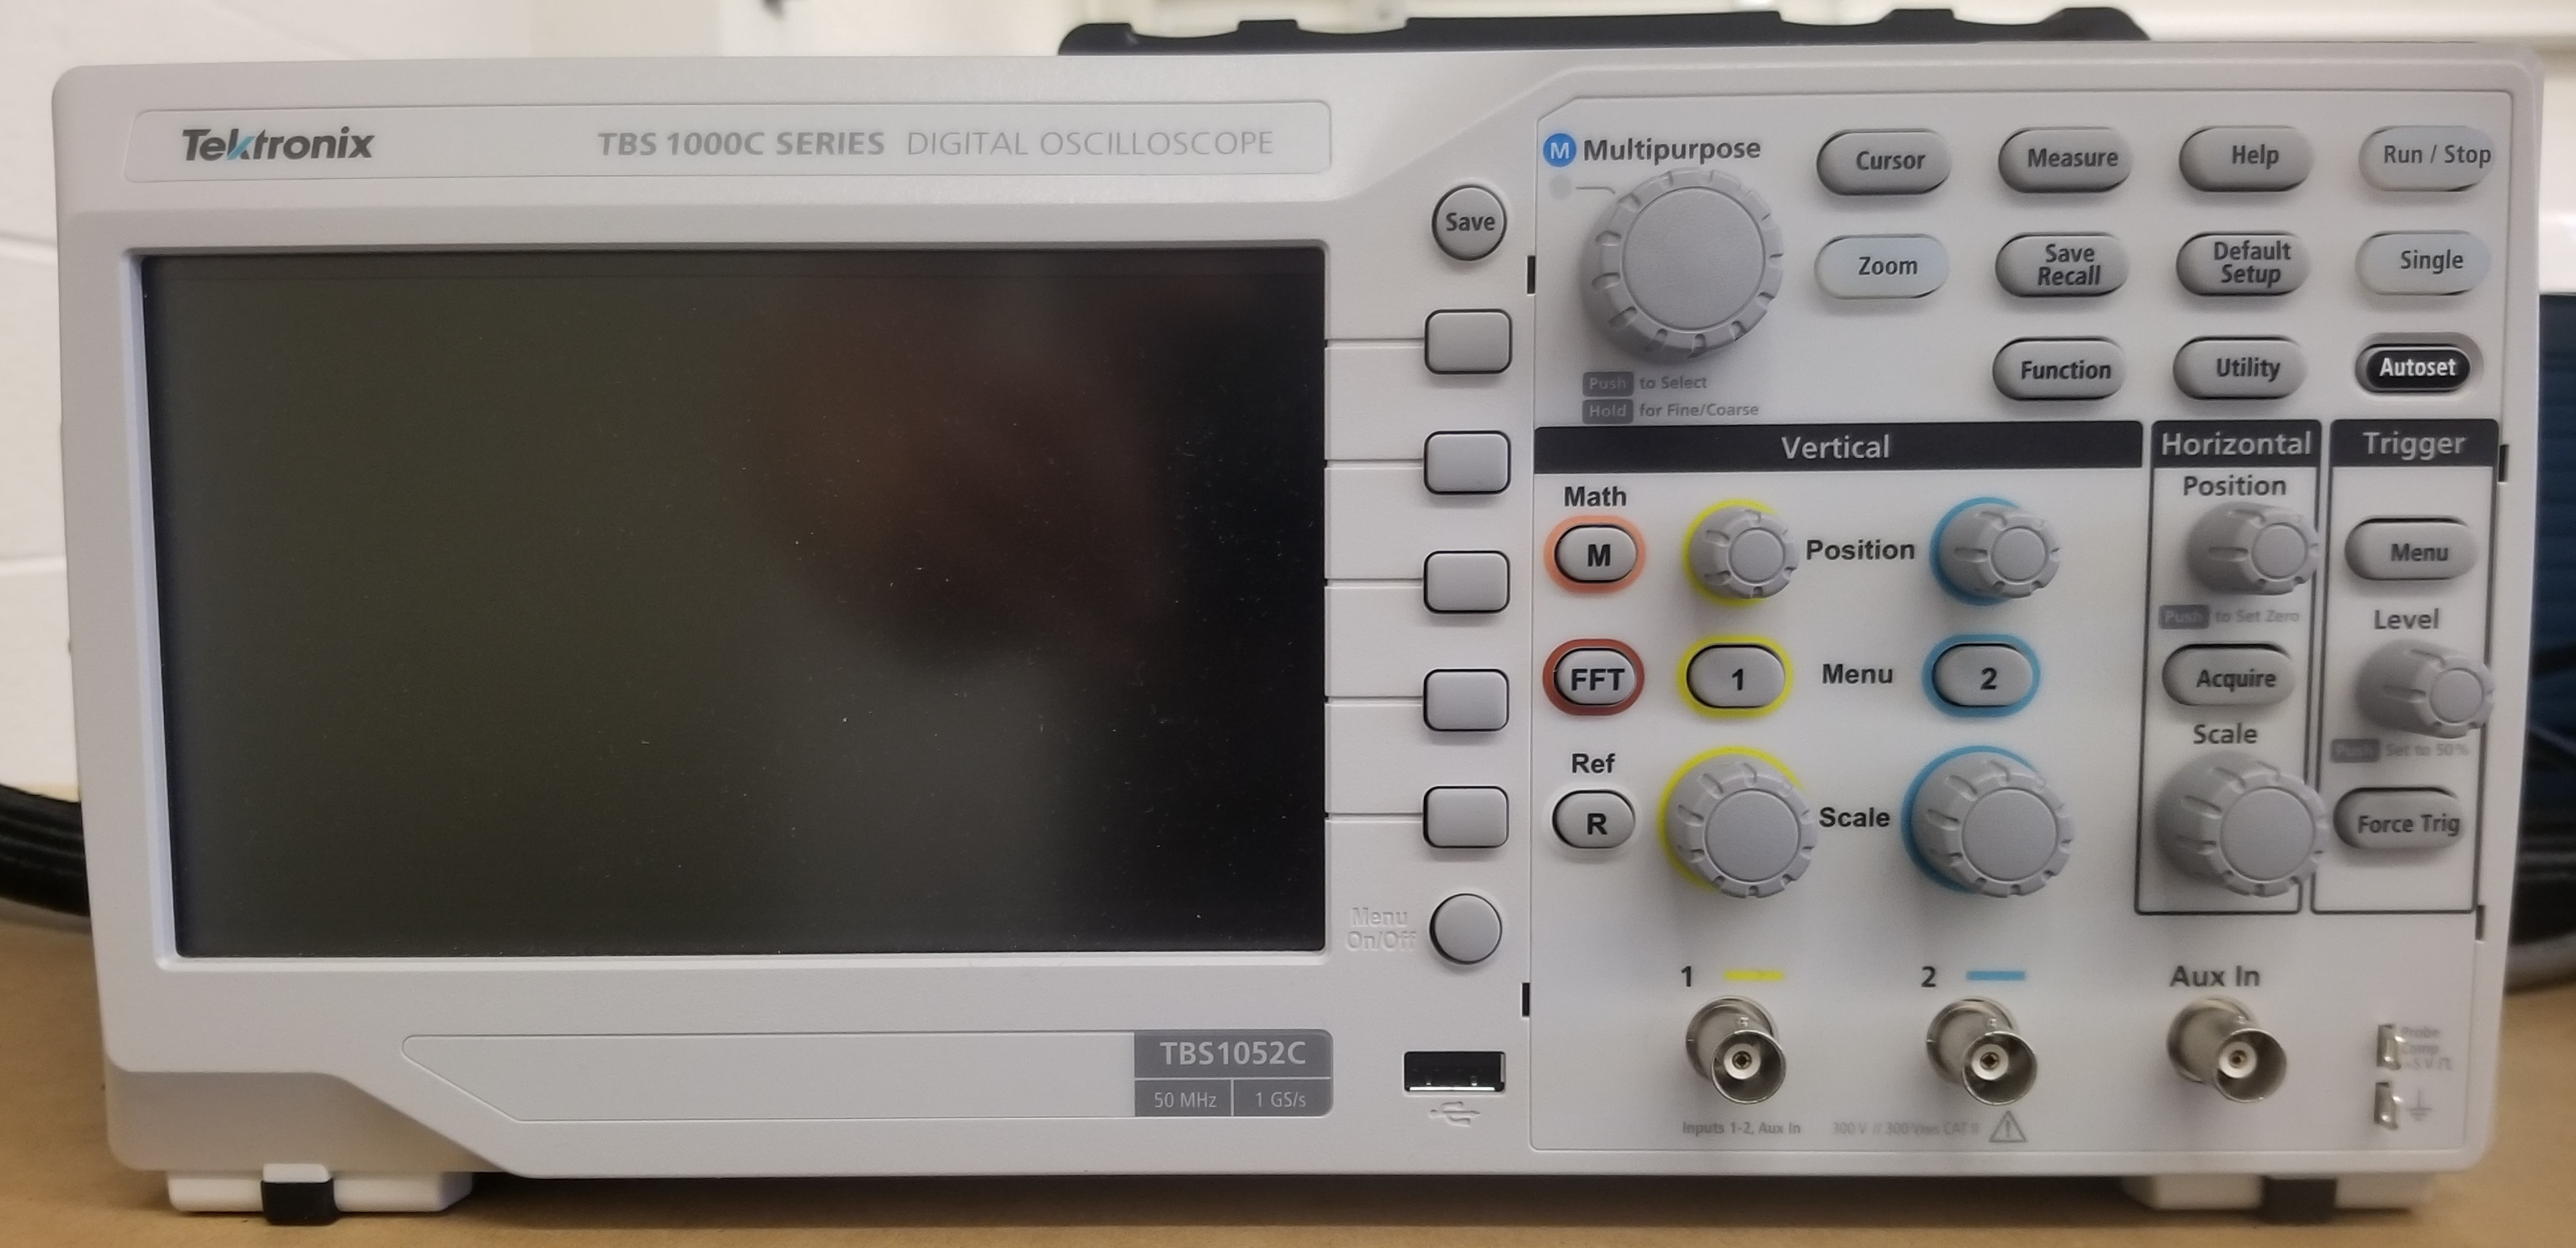
\includegraphics[scale=.025]{tektronix_tbs1000c_cropped.jpg}  \vspace{10mm}\\
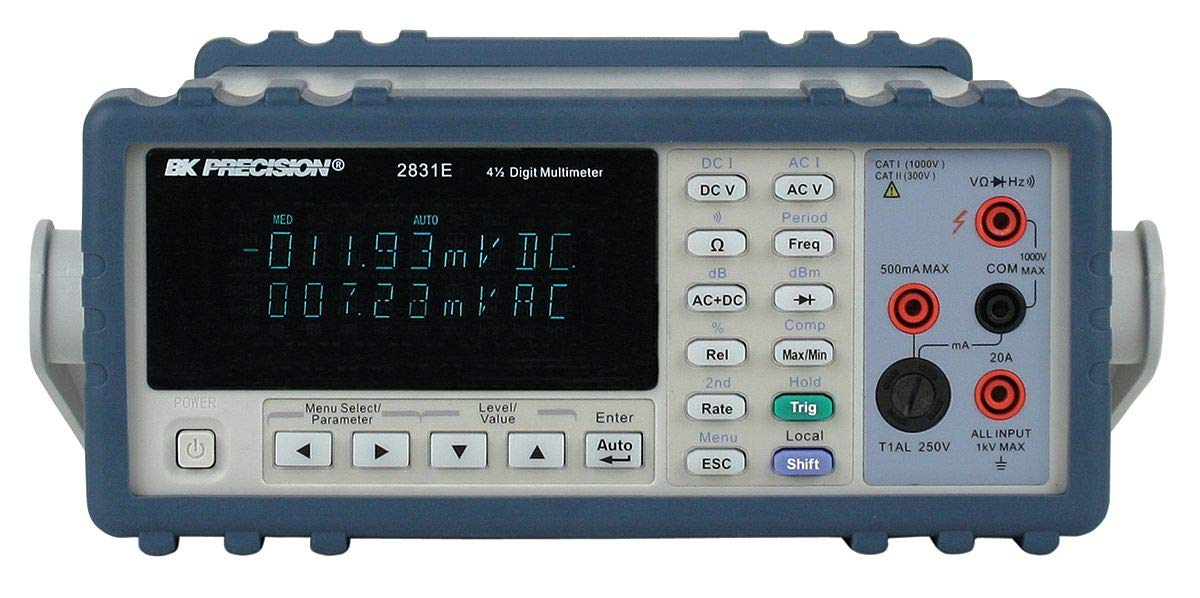
\includegraphics[scale=.10]{bk_2831e.jpg} \hspace{15mm} 
\includegraphics[scale=.025]{breadboard_template.png} 

%\end{multicols}	


}

% Section IV - Frame I:
\frame{  \small
\frametitle{\sectiontitleIV}



}




\end{document}